\documentclass[11pt]{article}
\usepackage[utf8]{inputenc}
\usepackage{graphicx}
\graphicspath{ {images/} }
\usepackage{geometry}
\geometry{a4paper}

\begin{document}

\section{19th of February}
\begin{itemize}
\item[•] We started by going over the feedback for the initial report. We came to the conclusion that the feedback wasn't very helpful. We haven't gotten a grade for the report.
\item[•] We discussed further how to implement the drivers behaviour class. We came to the conclusion that we would have a separate drivers class which would implement some of the methods that are currently in the vehicle class: optimalAcceleration, optimalDeceleration, etc. We would have three different kinds of drivers: reckless, normal, cautious. Delete the recklessBus, reckelessCar, etc. classes.
\item[•] We decided using test driven development (TDD) to some extend. Write tests that fail and work on the methods until every test passes.
\item[•] We discussed how to implement the traffic lights in detail. We decided that every junction should have a traffic light. And, to begin with, if there is green on one lane every other lanes at that junction should have a red light. Later we can implement some more advanced logic (left-hand-side rule).
\item[•] We discussed that every lane should have a width and the width of the road would be determined by number of lanes in that road.
\item[•] We discussed having more that one map a user can choose from to run the simulation, perhaps three different maps. First map would be really simple (one simple junction), second more complex and the third one the most complex.
\item[•] As the system is right now traffic accidents can happen, two vehicles can crash. We discussed that if that happens the ambulance can arrive at that scene and then will the crashed vehicles disappear. The crash will cause traffic jam, so if the ambulance cannot get to the crash the crashed vehicles will disappear in some time. This is just an idea and we will discuss this in more detail later.
\item[•] We allocated work among members:
	\begin{description}
	\item[Bálazs: ]Implement how cars are generated and enter and exit the system. Add some kind of feature that calculates how long each vehicle was in the system that will be logged.
	\item[Eddy: ]Continue working on the traffic lights and the drivers behaviour class.
	\item[Gabb: ]Do some further work on the GUI:
	\begin{itemize}
		\item[•] Have buses as a different image than cars.
		\item[•] Have cars and buses proportional to the sizes defined in the cars and buses class. 
		\item[•] Start to think about how to implement the user interface; buttons and boxes and stuff to set duration and what policy, etc.
		\item[•] And other stuff you can think of.
	\end{itemize}
	\item[Neab: ] Start work on the final report. There is a .tex file in the LaTeX directory in our repository on github called finalReport.tex. Please make all your changes in that file:
	\begin{itemize}
		\item[1.] cd to the correct directory in your computer, open terminal and write i.e: 
		\begin{verbatim}
		cd home/documents/trafficSimulator
		\end{verbatim}
		\item[2.] Pull the latest changes to your computer:
		\begin{verbatim}
		git pull
		\end{verbatim}
		\item[3.] Create a new branch called finalReport\_NeabInitialWork: 
		\begin{verbatim}
		git branch finalReport_NeabInitialWork
		\end{verbatim}
		\item[4.] Switch to the new branch:
		\begin{verbatim}
		git checkout finalReport_NeabInitialWork
		\end{verbatim}
		\item[5.] Now you can make your changes in Texmaker.
		\item[6.] Add the files you just edited:
		\begin{verbatim}
		git add LaTeX/finalReport.tex
		git add LaTeX/finalReport.pdf
		\end{verbatim}
		\item[7.] Commit theses changes:
		\begin{verbatim}
		git commit -m "Some message about the change"
		\end{verbatim}
		\item[8.] Push your branch to the origin:
		\begin{verbatim}
		git push origin finalReport_NeabInitialWork
		\end{verbatim}
		\item[9.] Then someone else should make a pull request and merge these changes to the master on github.
	\end{itemize}
	\item[Snorri: ]Implement the width of the lanes. Make more tests.
	\end{description}	 
\end{itemize}

 

\section{11th of February}
After the initial report presentation we had a short meeting where we discussed the next steps. We allocated tasks until next meeting. Bálazs was going to work on lane changing and collision detection for the vehicles. Eddy was going to work on creating a drivers class and a new architecture for the vehicles and traffic lights at junctions. Gabb was going to work on the gui. Neab was going to start the final report and think about the different traffic management policies. Snorri was going to do some testing. 

\section{9th of February}
We went over the initial report as a whole and made a few minor changes. Neab suggested a more rigorous timetable which is something we should consider for the final report.

We discusses what should be in the presentation. We decided to start with a short overview of the initial report, then show a class diagram and a use case diagram. And finish with a demo of the program. Neab was going to finish the presentation but he needed the diagrams from Eddy and was going to contact Gabb to get the first prototype running on his computer. Neab was going to check if the presentation works on his computer with in the room where the presentation is held.

We also discussed a better implementation of the cars and buses and drivers. Where we would have a different drivers class. Eddy was going to push a suggestion of improvement to some branch on github (I think).

\section{5th of February}
We discussed the resent additions we had made on the simulator, multiple vehicles and the GUI. The drives should have different behaviour, reckless driver on a bus or a car but not reckless car and a reckless bus.

Then we discusses the initial report and read the initial report handout. We decided to go with Mandatory/Optional table with 3 or 4 iterations. We discussed what our objectives were for this project.

We discussed whether we should have presentation slides and decided to have two slides, one would be the summary of the initial report and the other would be a UML diagram. We decided to meet on Monday 9th of feb to finish the initial report and presentation.

\newpage

\section{29th of January 2015}
\begin{itemize}
\item We discussed the the structure of the initial report and then revised the progress so far on the initial report. We discussed in particular what role each member should have, what project management style we should use and strategy.
\item We decided to use Trello for task management.
\item Roles: Bálazs - (lead) programmer, Gabb - (lead) graphical designer, Eddy - (lead) software architect, Neab - Project manager and Snorri - (lead) tester. So each member would supervise his sector of the project; for instance Eddy could make some unit test bench but Snorri would oversee all the tests and make sure that everything would be tested, etc.
\item We discussed some branching strategies on github. 
\end{itemize} 

\newpage

\section{21st of January 2015}
We discussed more technical aspects of the implementation; what classes we would create and their interrelation, what GUI platform we would use, how we would implement tests and when to start the test phase and if one of us should have the role of a tester, what IDE is nice, how Github works, ect. We decided that we would use a project management style built on iterations, start with building a simple prototype and try move closer towards the final product in each iteration. Finally we allocated work among ourselves unit next meeting:
\begin{itemize}
\item \textbf{Everyone:} Think about how to implement the project.

\item \textbf{Balázs:} Creating a project and making the first lines of code and put on Github.

\item \textbf{Eddy:} Creating a first draft of a UML diagram.

\item \textbf{Gabb and Neab:} Familiarise themselves with Github and GUI implementation with JavaFX.

\item \textbf{Snorri:} Write meeting log, and start the initial report.

\end{itemize} 

\newpage

\section{19th of January 2015}
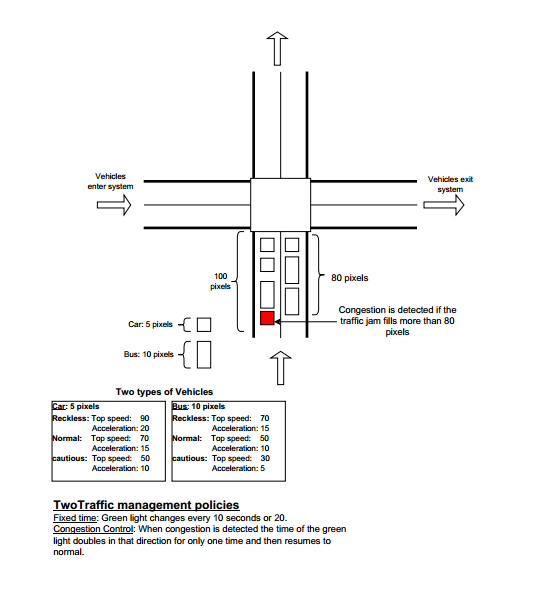
\includegraphics{meeting2}
\newpage

\section{15th of January 2015}
The project was introduced and the group was formed and we exchanged basic information about ourselves. We decided that we would use Java and discussed the time of next meeting. And decided that we would meet every Thursday at 10 o'clock.
\subsection{Members:}
\begin{itemize}
\item Balázs Kiss
\item Eddy Mukasa
\item Gabb Visessmit
\item Pongsakorn N. Riyamongkol
\item Snorri Hannesson
\end{itemize}
\newpage


\end{document}